\documentclass{beamer}

\usepackage{epsfig}
\usepackage{multicol}
\usepackage{geometry}
%\usepackage[dvipsnames]{xcolor}
\usepackage{textcomp}
\usepackage{graphicx}
\usepackage{caption}
\usepackage{subcaption}
\usepackage{amsmath}
\usepackage{tcolorbox}
\usetheme{Boadilla}
\usepackage{pict2e}
\usepackage{tikz}
\usepackage{xcolor}


\title[Traitement du signal numérique]{Traitement du signal numérique - HEI4 IMS}
\author[Antony Bazir]{}

\begin{document}

\begin{frame}
\frametitle{Notion de filtre}
\textbf{Qu'est ce qu'un filtre ? }\\
\only<2->
{
\vspace{1 cm}
\begin{center}
	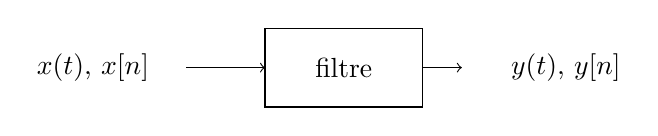
\begin{tikzpicture}

	\draw (2.15,0) node[left] {$x(t)$, $x[n]$};

	
	\draw[->] (2.5,0)-- (3.5,0);
	\draw (3.5,-0.5) rectangle(5.5,0.5) ;
	\draw (4.5,0) node {filtre};

	\draw[->] (5.5,0)-- (6,0);

	\draw (6.5,0) node[right] {$y(t)$, $y[n]$};

	\end{tikzpicture}
\end{center}
}

\only<3->{
\vspace{1 cm}
\begin{block}{}
"En traitement du signal, un filtre est un dispositif ou un processus permettant de retirer des composantes ou des parties indésirables d'un signal." (wikipedia.org)
\end{block}
}
\end{frame}

\subsection{Caractérisation de filtres}
\begin{frame}
\frametitle{Comment caractérise-t-on un filtre ?}
\textbf{Quels termes utiliseriez-vous pour définir un filtre ?}
\vspace{1cm}
\begin{itemize}
\item<2-> Analogique/Numérique
\vspace{0.2cm}
\item<3-> Actif/Passif (analogique)
\vspace{0.2cm}
\item<4-> Causal/Non causal (numérique)
\vspace{0.2cm}
\item<5-> Linéaire/Non linéaire 
\vspace{0.2cm}
\item<6-> Invariant/Non invariant dans le temps
\end{itemize}
\only<7->
{
\begin{block}{}
Objet du cours: Filtres numériques, causaux, linéaires, invariants dans le temps.
\end{block}
}
\end{frame}



\subsection{Linéarité}
\begin{frame}
\frametitle{Notion de linéarité}
\textbf{Question: Que veut dire linéaire en ingénierie des systèmes/automatique/traitement du signal ? \label{linéaire ?} }\\
\vspace{1 cm}
\only<2->
{
Soit $f : x \in \mathbb{R} \rightarrow f(x) \in \mathbb{R} $ et $(x_1,x_2,a,b) \in \mathbb{R}^4$
\\}
\vspace{1 cm}
\only<3->
{
$f$ linéaire si\\
\vspace{0.5 cm}

\[\boxed{f(a x_1 + b x_2) = a f(x_1) + b f(x_2)}\]

}

\end{frame}

\begin{frame}
\frametitle{Notion de linéarité}
 \textbf{Linéarité : application}
\textbf{Soit $x$ une variable réelle, les fonctions suivantes sont-elles linéaires ?}:
 \vspace{0.5cm}
\begin{itemize}
\item<2-> $f(x) = a x^2 + b x + c$ (avec $a$, $b$ et $c$ des constantes réelles positives)
\vspace{0.2cm}
\item<3-> $f(x) = \sqrt{x^2}$
\vspace{0.2cm}
\item<4-> $f(x) = a$ (constante réelle positive)
\vspace{0.2cm}
\item<5-> $f(x) = \ln(x)$
\vspace{0.2cm}
\item<6-> $f(x) = \frac{1}{a x + b}$
\end{itemize}
\vspace{1cm}
\only<8->
{
Aucune de ces fonctions n'est linéaire...
}
\end{frame}

\begin{frame}
\frametitle{Notion de linéarité: capteurs}
\textbf{Que vous évoque la notion de linéarité dans le cadre des capteurs ?}\\
\vspace{1 cm}
\only<2->{
\usetikzlibrary {decorations.pathmorphing} 
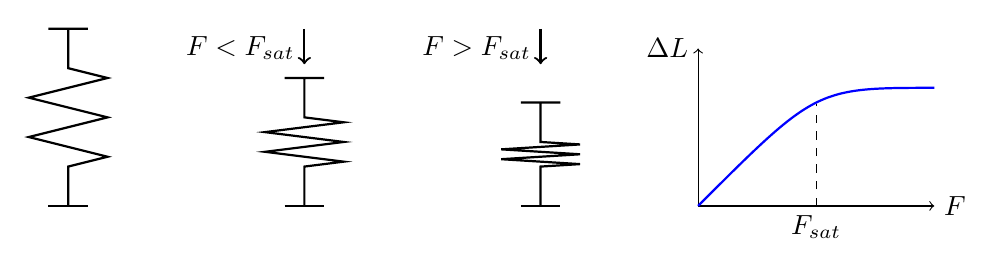
\begin{tikzpicture}

	%spring 
	\draw[thick] (-0.25,0)--(0.25,0);
	\draw[thick] (0,0)--(0,0.5)--++(0.5,0.125) --++(-1,0.25) --++(1,0.25) --++(-1,0.25) --++(1,0.25) --++(-0.5,0.125)--++(0,0.5)--++(-0.25,0)--++(0.5,0); 
		
%			\begin{scope}[xshift = 1.5cm]
%				\draw[thick,<->] (0,2.25)--(0,1.75); 
%				\draw (0,2) node[left] {$\Delta L$};
%			\end{scope}		
		
		
			\begin{scope}[xshift = 3cm]
			\draw[thick] (-0.25,0)--(0.25,0);
			\draw[thick] (0,0)--(0,0.5)--++(0.5,0.125/2) --++(-1,0.25/2) --++(1,0.25/2) --++(-1,0.25/2) --++(1,0.25/2) --++(-0.5,0.125/2)--++(0,0.5)--++(-0.25,0)--++(0.5,0); 
	\end{scope}
	
			\begin{scope}[xshift = 3cm]
				\draw[thick,->] (0,2.25)--(0,1.80); 
				\draw (0,2) node[left] {$F<F_{sat}$};
			\end{scope}	
	
	
	\begin{scope}[xshift = 6cm]
	\draw[thick] (-0.25,0)--(0.25,0);
			\draw[thick] (0,0)--(0,0.5)--++(0.5,0.125/4) --++(-1,0.25/4) --++(1,0.25/4) --++(-1,0.25/4) --++(1,0.25/4) --++(-0.5,0.125/4)--++(0,0.5)--++(-0.25,0)--++(0.5,0); 
	\end{scope}
	
		\begin{scope}[xshift = 6cm]
				\draw[thick,->] (0,2.25)--(0,1.80); 
				\draw (0,2) node[left] {$F>F_{sat}$};
			\end{scope}	
	

	
	\begin{scope}[xshift= 8cm] 
	\draw[->] (0,0)--(3,0) node[right] {$F$};
	\draw[->] (0,0)--(0,2) node[left] {$\Delta L$};	
	\draw[thick,blue] (0,0) .. controls (1.5,1.5) .. (3,1.5);
	\draw[dashed,black] (1.5,0)node[below]{$F_{sat}$} --(1.5,1.3) ;
	\end{scope}
\end{tikzpicture}
}
\only<3->{
\begin{block}{}
Le capteur sort de sa zone de linéarité lorsqu'on perd la relation linéaire/affine entre l'entrée et la sortie
\end{block}
}
\end{frame} 



\subsection{Invariance dans le temps}
\begin{frame}
\frametitle{Notion d'invariance dans le temps}
Prérequis : Notion de retard d'une fonction \\
\only<2->{
\vspace{1 cm} 
Soit $x : t \in \mathbb{R} \rightarrow x(t) \in \mathbb{R} $ \\

\vspace{1 cm} 
La fonction $x(t)$ retardée de $\tau \in \mathbb{R}$ s'écrit $x(t-\tau)$\\
\vspace{1 cm}
}

\only<3->{
La suite $x[n]$ retardée de $k \in \mathbb{N}$ s'écrit $x[n-k]$
}

\end{frame}

\begin{frame}
\frametitle{Invariance dans le temps}

\begin{block}{Attention}
La notion d'invariance dans le temps est ici appliqué au \textbf{filtre/système} faisant la correspondance entre les \textbf{fonctions} d'entrée et de sortie 
\end{block}
\end{frame}


\begin{frame}
\frametitle{Invariance dans le temps}
Soit $F$ un filtre de telle sorte que, pour $x(t)$ et $y(t)$ deux fonctions , $ \forall \; t \in \mathbb{R}, \; y(t) = F(x(t))$ ou $ \forall \; n \in \mathbb{N}, \; y[n] = F(x[n])$ \\

\only<2->
{
\vspace{1cm} 
le filtre $F$  est dit \textbf{invariant dans le temps} si \\
\vspace{1cm}
\begin{center}
$\forall \tau \in \mathbb{R}, \;\; F(x(t-\tau)) = y(t-\tau)$\\
\vspace{0.7 cm}
$\forall k \in \mathbb{N}, \;\; F(x[n-k]) = y[n-k]$\\
\end{center}
}

\only<3->
{ 
\begin{block}{}
	En résumé, la réponse d'un filtre/système invariant dans le temps ne doit pas dépendre du moment où on l'utilise
\end{block} 
}

\end{frame}


\subsection{Système linéaire et invariant dans le  temps (LIT)}

\begin{frame}
\frametitle{Système linéaire et invariant dans le  temps (LIT) }

Un système $F$ est linéaire et invariant dans le temps (LIT) si :
\vspace{0.3cm}
\begin{itemize}
\item La sortie correspondant à une combinaison linéaire de signaux d'entrée est la combinaison linéaire des signaux de sortie correspondant aux entrées prises séparément\\
\vspace{0.3cm}
\item la réponse d'un filtre/système invariant dans le temps ne doit pas dépendre du moment où on l'utilise\\
\end{itemize}

\end{frame} 

\begin{frame} 
\frametitle{Système linéaire et invariant dans le temps (LIT) }
Soit un signal d'entrée $x$ (continu ou discret) et $F$ un filtre/système LIT\\
\vspace{1 cm}
\begin{columns}
\column{65mm}
\begin{center}
$x(t) = \displaystyle \int x(\tau)  \; \delta(t-\tau) \; d\tau$\\
\only<2->{
\vspace{0.5cm}!
$F(x(t)) = y(t)$\\
$ = F( \displaystyle \int x(\tau)\;  \delta(t-\tau) \; d\tau)$\\
\vspace{0.5cm}
}

\only<3->{
F linéaire donc, \\
\vspace{0.5cm}
$F(x(t)) = y(t) $\\
$= \displaystyle \int F (x(\tau) \; \delta(t-\tau) \; d\tau)$
}
\end{center}

\column{55mm}
\begin{center}
$x[n] =  \displaystyle \sum \; x[k] \; \delta[n-k] $ \\
\vspace{0.5cm}

\only<2->{
$F(x[n]) = y[n] $\\

$= F(\displaystyle \sum \; x[k] \;  \delta[n-k]) $ \\
\vspace{0.5cm}
}

\only<3->{
F linéaire donc, \\
\vspace{0.5cm}
$F(x[n]) = y[n] $\\
$ = \displaystyle \sum F( x[k] \; \delta[n-k]) $ \\
}

\end{center}
\end{columns}
\end{frame}

\begin{frame} 
\frametitle{Système linéaire et invariant dans le temps (LIT) }
Soit un signal d'entrée $x$ (continu ou discret) et $F$ un filtre/système LIT\\
\vspace{1 cm}
\begin{columns}
\column{65mm}
\begin{center}
$F(x(t)) = y(t) $\\
$= \displaystyle \int F (x(\tau) \; \delta(t-\tau) \; d\tau)$\\
\vspace{0.5cm}

$F$ s'applique aux fonctions de $t$\\
\vspace{0.5cm}

$y(t) = \displaystyle \int x(\tau) \; F(\delta(t-\tau) \; )d\tau$\\
\vspace{0.5cm}

\end{center}

\column{55mm}
\begin{center}
$F(x[n]) = y[n] $\\
$ = \displaystyle \sum \; F( x[k] \; \delta[n-k]) $ \\
\vspace{0.5cm}

$F$ s'applique aux suites sur $n$\\
\vspace{0.5cm}

$ y[n] = \displaystyle \sum \; x[k] \;  F(\delta[n-k]) $ \\
\vspace{0.5cm}


\end{center}
\end{columns}
\end{frame}

\begin{frame} 
\frametitle{Système linéaire et invariant dans le temps (LIT) }
Soit un signal d'entrée $x$ (continu ou discret) et $F$ un filtre/système LIT\\
\vspace{1 cm}
\begin{columns}
\column{65mm}
\begin{center}
$y(t) = \displaystyle \int x(\tau) \; F(\delta(t-\tau) ) \;d\tau$\\
\vspace{0.5cm}

Puisque $F$ invariant dans le temps,\\
\vspace{0.5cm}

$y(t) = \displaystyle \int x(\tau) \; h(t-\tau) \; d\tau$\\
\vspace{0.5cm}

avec $h[t]$ la\\ \textbf{réponse impulsionnelle} du filtre $F$

\end{center}

\column{55mm}
\begin{center}

$ y[n] = \displaystyle\sum x[k]  F(\delta[n-k]) $ \\
\vspace{0.5cm}

Puisque $F$ invariant dans le temps,\\
\vspace{0.5cm}

$ y[n] = \displaystyle\sum x[k]  h[n-k] $ \\
\vspace{0.5cm}

avec $h[n]$ la\\ \textbf{réponse impulsionnelle} du filtre $F$

\end{center}
\end{columns}
\begin{block}{}
Ces deux relations sont ce qu'on appelle \textbf{l'équation de convolution}
\end{block}
\end{frame}

\begin{frame}
\frametitle{Système linéaire et invariant dans le temps (LIT)}
Le fait que le sytème soit LIT et les équations de convolution sous-tendent: \\
\vspace{1cm}
\begin{itemize}
\item La possibilité d'écrire une \textbf{fonction de transfert}
\vspace{0.3cm}
\item La possibilité de \textbf{prédire/calculer le comportement} d'un système "arbitraire"
\vspace{0.3cm}
\item La possibilité de créer des \textbf{systèmes complexes} au comportement connu à partir de \textbf{cellules "simples"}
\end{itemize}

\end{frame} 

\section{Filtres numériques}
\subsection{Définition}
\begin{frame}
\frametitle{Définir un filtre numérique}
Il existe trois façons équivalentes de définir un filtre numérique :\\
\vspace{0.5cm}
\begin{columns}[T]
\column{40mm}
\only<2->{
Equation de récurrence :\\
\vspace{1cm} 
\small \[ y[n] = x[n] + a y[n-1]\]
}
\column{40mm}
\only<3->{
Fonction de transfert :\\
\vspace{1cm}
\small \[ H(z) = \frac{Y(z)}{X(z)} = \frac{z}{z-a} \]
} 
\column{40mm}
\only<4->{
Réponse impulsionnelle:\\
\vspace{1cm}
\small \[ h[n] = a^{n} \]
}
\end{columns}
\end{frame}

\begin{frame}
\frametitle{Définir un filtre numérique}
\begin{center}
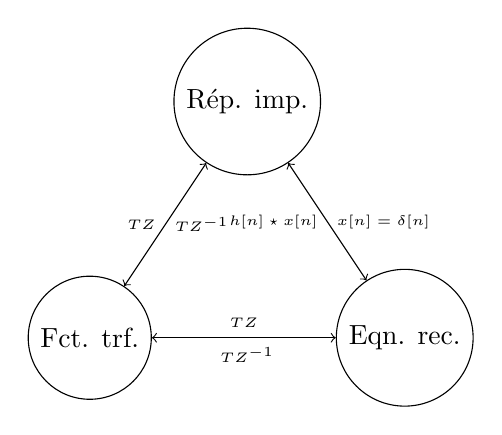
\begin{tikzpicture}
		\node[circle,draw] (E) at (2,0) {Eqn. rec.};
		\node[circle,draw] (F) at (-2,0) {Fct. trf.};
		\node[circle,draw] (R) at (0,3) {Rép. imp.};
		
		\draw[<->] (E)node[below, midway] {\tiny $TZ^{-1}$} --(F) node[above, midway] {\tiny  $TZ$};
		\draw[<->] (F) --(R)node[right, midway] {\tiny $TZ^{-1}$} node[left, midway] {\tiny $TZ$} ; 
		\draw[<->] (R) --(E) node[right, midway] {\tiny $x[n]=\delta [n]$} node[left, midway] {\tiny $h[n]\star x[n]$};
		
		%\draw (0,-0.3) node {$TZ$};
		%\draw (0,0.3) node {$TZ^{-1}$};
		
		%\draw (0.6,1.5) node {$h[n]\star x[n]$};
		%\draw (1.4,1.5) node {$x[n]=\delta [n]$};
		
		%\draw (-1,1.5) node {$TZ$};
		%\draw (-3,1.5) node {$TZ^{-1}$};
\end{tikzpicture}
\end{center}

\end{frame}

\subsection{Fonction de transfert, équation de récurrence et réponse impulsionnelle: Exemples}

\begin{frame}
\frametitle{Exemple de définition d'un filtre}
On part de l'équation de récurrence:   $ y_1[n] = \frac{\displaystyle x_1[n] + x_1[n-1]}{\displaystyle 2}$\\
\vspace{0.3cm}
Fonction de transfert : 
\vspace{0.2cm}

\only<2->{
\[ y_1[n] = \frac{x_1[n] + x_1[n-1]}{2}  \; -\boxed{TZ} \;  \rightarrow Y_1(z) = \frac{X_1(z) + X_1(z)z^{-1}}{2} \]
}
\vspace{0.2cm}

\only<3->{
\[ Y_1(z) = \frac{X_1(z) + X_1(z)z^{-1}}{2} \rightarrow Y_1(z) = X_1(z)\frac{(1 + z^{-1})}{2}  \]
}

\vspace{0.3cm}
\only<4->{
\[ \boxed{ \rightarrow \frac{Y_1(z)}{X_1(z)} = H_1(z) = \frac{(1 + z^{-1})}{2}}  \]
}

\end{frame}

\begin{frame}
\frametitle{Exemple de définition d'un filtre}
On part de l'équation de récurrence:   $ y_1[n] = \frac{\displaystyle x_1[n] + x_1[n-1]}{\displaystyle 2}$\\ 
\vspace{0.2cm}
Réponse impulsionnelle : 
\vspace{0.2cm}
On remplace $x_1[n]$ par $\delta[n]$\\
\vspace{0.2cm}

\only<2->{
\[ y_1[n] = \frac{x_1[n] + x_1[n-1]}{2}  \; -\boxed{\delta[n]}\rightarrow \;  h_1[n] = \frac{\delta[n] + \delta[n-1]}{2} \]
}
\vspace{0.2cm}

\only<3->{
\begin{center}
\begin{tikzpicture}
\draw[->] (-2,0)--(2,0) node[right] {$n$};
\draw[->] (0,0)--(0,1.2) node[above] {$h[n]$};

\draw[->,thick,blue] (-2,0)--(-2,0);
\draw[->,thick,blue] (-1,0)--(-1,0);
\draw[->,thick,blue] (0,0)--(0,0.5);
\draw[->,thick,blue] (1,0)--(1,0.5);
\draw[->,thick,blue] (2,0)--(2,0);
\end{tikzpicture}
\end{center}

}

\end{frame}

\begin{frame}
\frametitle{Exemple de définition d'un filtre}
On part de la fonction de transfert : $H_2(z) = \frac{\displaystyle z}{\displaystyle (z-1) }$\\
\vspace{0.3cm}

\only<2->{
\[H_2(z) = \frac{ z}{ z-1 } =\frac{1}{(1 - z^{-1})}\]
}
\vspace{0.3cm}
\only<3->{
\[H_2(z) = \frac{Y_2(z)}{X_2(z)}  =\frac{1}{(1 - z^{-1})}\]
}
\vspace{0.3cm}
\only<3->{
\[Y_2(z)(1 - z^{-1})  = X_2(z)\]
}

\end{frame}

\begin{frame}
\frametitle{Exemple de définition d'un filtre}
\[ Y_2(z)(1 - z^{-1})  = X_2(z)  = Y_2(z) - Y_2(z)z^{-1}  \]\\
\vspace{0.3cm} 
On repasse en temporel,
\\
\vspace{0.2cm}

\only<2->{
\[ Y_2(z) - Y_2(z)z^{-1} = X_2(z) -\boxed{TZ^{-1}} \rightarrow  y_2[n] - y_2[n-1] = x[n] \]
}

\vspace{0.3cm}
\only<3->{
\[ \boxed{H_2(z) = \frac{z}{z-1 } \rightarrow  y_2[n] = x_2[n]+y_2[n-1] }\]
}

\end{frame}

\subsection{Réponse en fréquence: Premier exemple}
\begin{frame}
\frametitle{Réponse en fréquence de filtres numériques}
\underline{Important :} Lorsqu'on parle de la réponse en fréquence d'un filtre, on fait référence à sa \textbf{transformée de Fourier.}\\
\vspace{0.3cm}

\only<2->{
Comme en continu, changement de variable pour passer dans le domaine de Fourier:\\

\vspace{0.2cm}
\[ z = e^{2 j \pi \nu T_e}  \] 
}

\vspace{0.4cm}
\only<3->{
Reprenons les filtres précédents
}
\end{frame}

\begin{frame}
\frametitle{Réponse en fréquence de filtres numériques} 
\[ y_1[n] = \frac{x_1[n] + x_1[n-1]}{2}  \; \rightarrow \; H_1(z) = \frac{(1 + z^{-1})}{2} \]

\vspace{0.3cm}
\only<2->{
\[H_1(z) = \frac{(1 + z^{-1})}{2} \rightarrow  H_1(\nu) = \frac{(1 + e^{-2 j \pi \nu T_e})}{2} \]
}
\vspace{0.3cm}
\only<2->{
\[H_1(\nu) = \frac{(1 + e^{-2 j \pi \nu T_e})}{2} =  e^{- j \pi \nu T_e} \frac{(e^{ j \pi \nu T_e} + e^{- j \pi \nu T_e})}{2} \]
}

\vspace{0.3cm}
\only<3->{
\[\boxed{H_1(\nu) =   \cos(\pi \nu T_e)e^{- j \pi \nu T_e}} \]
}
\end{frame}

\begin{frame}
\frametitle{Réponse en fréquence de filtres numériques} 
\underline{Rappel} : Réponse en fréquence = Module + phase \\
\vspace{0.5cm}
\begin{columns}[T]
\column {60mm}
\only<2->{
\vspace{0.4cm}
\[|H_1(\nu)|  =   |\cos(\pi \nu T_e)| \]\\
}

\vspace{0.06cm}
\only<3->{
\begin{center}
\begin{tikzpicture}
\draw[->] (-2,0)--(2,0) node[right] { $\scriptstyle \nu$};
\draw[->] (0,0)node[below] {\scriptsize 0} -- (0,1.5) ;
\draw (0,2) node {$\scriptstyle |H_1(\nu)|$};
\draw (0.5,-0.4) node {$\frac{f_e}{2}$};

\draw[domain=-0.5:0.5,color=blue,samples=100] plot (\x,{abs(cos(3.14 *\x r))});
\draw[dashed,domain=-1.5:1.5,color=blue,samples=100] plot (\x,{abs(cos(3.14 *\x r))});
\end{tikzpicture}
\end{center}
}

\column{60mm}
\only<2->{
\[\textrm{arg}(H_1(\nu)) =  \arctan(\tan(\pi \nu T_e))  \]\\
}

%\vspace{0.5cm}


\only<3->{
\begin{center}
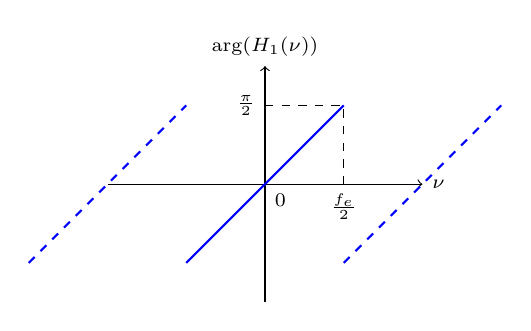
\begin{tikzpicture}
\draw[->] (-2,0)-- (2,0) node[right] {$\scriptstyle \nu$};
\draw[->] node[below right]{\scriptsize 0} (0,-1.5) -- (0,1.5) node[above] {$\scriptstyle \textrm{arg}(H_1(\nu))$} ;

\draw[thick,blue] (-1,-1)--(1,1); 
\draw[dashed,thick,blue] (-3,-1)--(-1,1); 
\draw[dashed,thick,blue] (1,-1)--(3,1);


\draw[dashed] (1,0) node[below] {$\scriptstyle \frac{f_e}{2}$} --(1,1) ;
\draw[dashed] (0,1) node[left] {$\scriptstyle \frac{\pi}{2}$} --(1,1)  ; 
\end{tikzpicture}
\end{center}

}
\end{columns}
\end{frame}

\begin{frame}
\frametitle{Réponse en fréquence de filtres numériques} 
La fonction de transfert possède un zéro en $\frac{\displaystyle f_e}{\displaystyle 2}$\\
\vspace{0.2cm}
\begin{columns}
\column{60mm}
\begin{center}
\begin{tikzpicture}
\draw[->] (-2,0)--(2,0) node[right] { $\scriptstyle \nu$};
\draw[->] (0,0)node[below] {\scriptsize 0} -- (0,1.5) ;
\draw (0,2) node {$\scriptstyle |H_1(\nu)|$};
\draw (0.5,-0.4) node {$\frac{f_e}{2}$};

\draw[domain=-0.5:0.5,color=blue,samples=100] plot (\x,{abs(cos(3.14 *\x r))});
\draw[dashed,domain=-1.5:1.5,color=blue,samples=100] plot (\x,{abs(cos(3.14 *\x r))});
\end{tikzpicture}
\end{center}

\column{60mm}
\only<2->{
\vspace{1.5cm}
\begin{center}
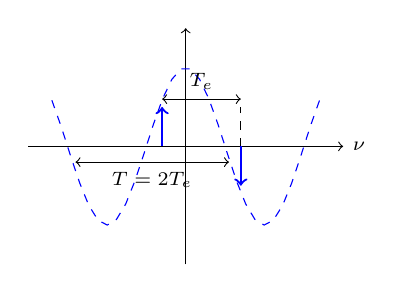
\begin{tikzpicture}
\draw[->] (-2,0)--(2,0) node[right] { $\scriptstyle \nu$};
\draw[->] (0,-1.5)-- (0,1.5) ;
%%\draw (0,2) node {$\scriptstyle |H_1(\nu)|$};
%%\draw (0.5,-0.4) node {$\frac{f_e}{2}$};
\draw[<->] (-1.4,-0.2)--(0.55,-0.2) node[midway,below]{\scriptsize $T = 2T_e$};
%
\draw[dashed,domain=-1.7:1.7,color=blue,samples=30] plot (\x,{cos(3.14 *\x r)});

\draw[->,thick,blue] (-0.3,0)--(-0.3,0.5);
\draw[->,thick,blue] (0.7,0)--(0.7,-0.5);
\draw[-,dashed] (0.7,0)--(0.7,0.5);
\draw[<->] (-0.3,0.6)--(0.7,0.6) node[midway,above]{\scriptsize $T_e$};
\end{tikzpicture}
\end{center}
}
\end{columns}
\vspace{0.5cm}
\only<3->{
Si le signal est de fréquence $f_e/2$ alors les échantillons prélevés sont toujours de signe oppopsés et s'annulent...
}


\end{frame}



\begin{frame}
\frametitle{Réponse en fréquence de filtres numériques} 
\[ H_1(\nu) =   \frac{(1 + z^{-1})}{2} \]
\begin{columns}[T]
\column {60mm}

\vspace{0.16cm}

\begin{center}
\begin{tikzpicture}
\draw[->] (-2,0)--(2,0) node[right] { $\scriptstyle \nu$};
\draw[->] (0,0)node[below] {\scriptsize 0} -- (0,1.5) ;
\draw (0,2) node {$\scriptstyle |H_1(\nu)|$};
\draw (0.5,-0.4) node {$\frac{f_e}{2}$};

\draw[domain=-0.5:0.5,color=blue,samples=100] plot (\x,{abs(cos(3.14 *\x r))});
\draw[dashed,domain=-1.5:1.5,color=blue,samples=100] plot (\x,{abs(cos(3.14 *\x r))});
\end{tikzpicture}
\end{center}


\column{60mm}



\begin{center}
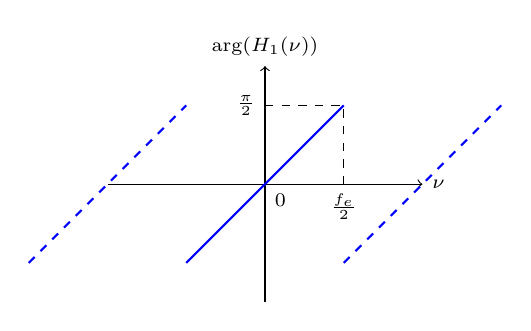
\begin{tikzpicture}
\draw[->] (-2,0)-- (2,0) node[right] {$\scriptstyle \nu$};
\draw[->] node[below right]{\scriptsize 0} (0,-1.5) -- (0,1.5) node[above] {$\scriptstyle \textrm{arg}(H_1(\nu))$} ;


\draw[thick,blue] (-1,-1)--(1,1); 
\draw[dashed,thick,blue] (-3,-1)--(-1,1); 
\draw[dashed,thick,blue] (1,-1)--(3,1);

\draw[dashed] (1,0) node[below] {$\scriptstyle \frac{f_e}{2}$} --(1,1) ;
\draw[dashed] (0,1) node[left] {$\scriptstyle \frac{\pi}{2}$} --(1,1)  ; 
\end{tikzpicture}
\end{center}


\end{columns}
\vspace{0.5cm}
\only<2->{
Et si on veut un filtre similaire que ne coupe pas en $f_e/2$ ?
}
\end{frame}

\begin{frame}
\frametitle{Réponse en fréquence de filtres numériques}
\[ H_1^*(\nu) =   \frac{(1 - z^{-1})}{2} \; \Leftrightarrow \; y_1^*[n] = \frac{x_1[n] - x_1[n-1]}{2}  \]

\begin{columns}
\column{60mm}
\only<2->{
\[ |H_1^*(\nu)| = |\sin(\pi \nu T_e)| \]
\begin{center}
\begin{tikzpicture}
\draw[->] (-2,0)--(2,0) node[right] { $\scriptstyle \nu$};
\draw[->] (0,0)node[below] {\scriptsize 0} -- (0,1.5) ;
\draw (0,2) node {$\scriptstyle |H_1*(\nu)|$};
\draw (0.5,-0.4) node {$\frac{f_e}{2}$};

\draw[domain=-0.5:0.5,color=blue,samples=100] plot (\x,{abs(sin(3.14 *\x r))});
\draw[dashed,domain=-1.5:1.5,color=blue,samples=100] plot (\x,{abs(sin(3.14 *\x r))});
\end{tikzpicture}
\end{center}

}

\column{60mm}
\only<2->{
\[ \textrm{arg}(H_1^*(\nu))= \arctan(\frac{1}{\tan( \pi \nu T_e)}) \]
\begin{center}
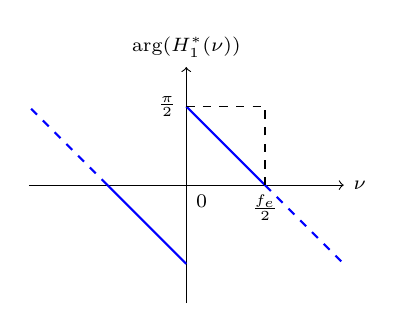
\begin{tikzpicture}
\draw[->] (-2,0)-- (2,0) node[right] {$\scriptstyle \nu$};
\draw[->] node[below right]{\scriptsize 0} (0,-1.5) -- (0,1.5) node[above] {$\scriptstyle \textrm{arg}(H_1^*(\nu))$} ;


\draw[thick,blue] (0,1)--(1,0);
\draw[thick,blue] (-1,0)--(0,-1); 
\draw[dashed,thick,blue] (1,0)--(2,-1); 
\draw[dashed,thick,blue] (-1,0)--(-2,1); 

\draw[dashed] (1,0) node[below] {$\scriptstyle \frac{f_e}{2}$} --(1,1) ;
\draw[dashed] (0,1) node[left] {$\scriptstyle \frac{\pi}{2}$} --(1,1)  ; 
\end{tikzpicture}
\end{center}
}
\end{columns}
\vspace{0.5cm}
\only<3->{
On voit que ce filtre ci va plutôt couper les composantes basses fréquences
}

\end{frame}


\subsection{Types de filtres}
\begin{frame}
\frametitle{Types de filtres numériques : Amplitude} 
\begin{columns}[T]
\column{30mm}
\only<2->{
\begin{center} 
Passe-bas :\\
\vspace{0.5cm}
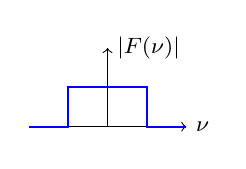
\begin{tikzpicture}
\draw[->] (0,0)--(0,1) node[right]{\footnotesize $|F(\nu)|$};
\draw[->] (-1,0)--(1,0) node[right]{ \footnotesize $\nu$};

\draw[thick,blue] (-1,0)--(-0.5,0)--(-0.5,0.5)--(0.5,0.5)--(0.5,0)--(1,0);
\end{tikzpicture}
\end{center}
}

\column{30mm}
\only<3->{
\begin{center} 
Passe-haut :\\
\vspace{0.5cm}
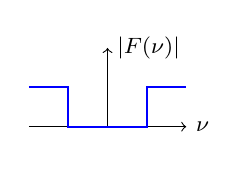
\begin{tikzpicture}
\draw[->] (0,0)--(0,1) node[right]{\footnotesize $|F(\nu)|$};
\draw[->] (-1,0)--(1,0) node[right]{\footnotesize $\nu$};

\draw[thick,blue] (-1,0.5)--(-0.5,0.5)--(-0.5,0)--(0.5,0)--(0.5,0.5)--(1,0.5);
\end{tikzpicture}
\end{center}
}

\column{30mm}
\only<4->{
\begin{center}
Passe-bande :\\
\vspace{0.5cm}

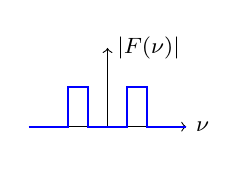
\begin{tikzpicture}
\draw[->] (0,0)--(0,1) node[right]{\footnotesize $|F(\nu)|$};
\draw[->] (-1,0)--(1,0) node[right]{\footnotesize $\nu$};

\draw[thick,blue] (-1,0)--(-0.5,0)--(-0.5,0.5)--(-0.25,0.5)--(-0.25,0)--(0.25,0)--(0.25,0.5)--(0.5,0.5)--(0.5,0)--(1,0);
\end{tikzpicture}
\end{center}
}

\column{30mm}
\only<5->{
\begin{center}
Coupe-bande :\\
\vspace{0.5cm}

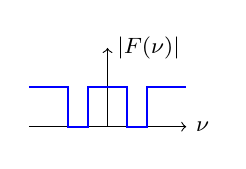
\begin{tikzpicture}
\draw[->] (0,0)--(0,1) node[right]{\footnotesize $|F(\nu)|$};
\draw[->] (-1,0)--(1,0) node[right]{\footnotesize $\nu$};

\draw[thick,blue] (-1,0.5)--(-0.5,0.5)--(-0.5,0)--(-0.25,0)--(-0.25,0.5)--(0.25,0.5)--(0.25,0)--(0.5,0)--(0.5,0.5)--(1,0.5);
\end{tikzpicture}
\end{center}
}
\end{columns} 
\vspace{1cm}
\only<6->{
On peut également définir des filtres "shelf" où on ne coupe pas complètement en dehors de la bande passante etc...
}
\end{frame}

\begin{frame}
\frametitle{Exemple d'utilisation : Filtre passe-bas}
\begin{columns}

\column{60mm}


\begin{center}
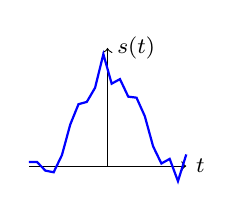
\begin{tikzpicture}
\draw[->] (0,0)--(0,1.5) node[right]{\footnotesize $s(t)$};
\draw[->] (-1,0)--(1,0) node[right]{\footnotesize $t$};
\draw[thick,blue] plot coordinates{(-5.00000/5,0.051378 )
 (-4.473684/5,0.051094) 
 (-3.947368/5,-0.057463)
 (-3.421053/5,-0.079000) 
 (-2.894737/5,0.139569)
  (-2.368421/5,0.526946)
   (-1.842105/5,0.786162) 
   (-1.315789/5,0.814761)
    (-0.789474/5,0.995006)
     (-0.263158/5,1.421068)
      (0.263158/5,1.046368)
       (0.789474/5,1.104432) 
       (1.315789/5,0.881924)
       (1.842105/5,0.868557) 
       (2.368421/5,0.633392)
        (2.894737/5,0.250564) (3.421053/5,0.032500) 
        (3.947368/5,0.091466) (4.473684/5,-0.191670) 
        (5.000000/5,0.147825) };
\end{tikzpicture}\\
\vspace{1cm}
\only<2->{
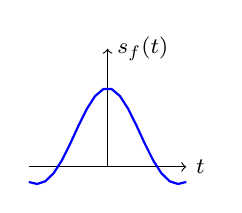
\begin{tikzpicture}
\draw[->] (0,0)--(0,1.5) node[right]{\footnotesize $s_f(t)$};
\draw[->] (-1,0)--(1,0) node[right]{\footnotesize $t$};
\draw[thick,blue] plot coordinates{
  (-1.000000,  -0.191785)
  (-0.894737, -0.217191)
  (-0.789474,  -0.182747)
  (-0.684211,  -0.080629)
  (-0.578947,   0.084414)
  (-0.473684,   0.294884)
  (-0.368421,   0.523000)
  (-0.263158,   0.735423)
  (-0.157895,   0.899311)
  (-0.052632,  0.988498)
  ( 0.052632,  0.988498)
  ( 0.157895,   0.899311)
  ( 0.263158,   0.735423)
  ( 0.368421,   0.523000)
  ( 0.473684,   0.294884)
  ( 0.578947,   0.084414)
  ( 0.684211,  -0.080629)
  ( 0.789474, -0.182747)
  ( 0.894737, -0.217191)
  ( 1.000000,  -0.191785)
 };
\end{tikzpicture}
}
\end{center}

\column{60mm}
\only<3->{
\begin{itemize}
\item Débruitage/Lissage 
\vspace{0.3cm}
\item Utilisé pour construire des filtres plus complexes
\end{itemize}
} 

\end{columns}

\end{frame}

\begin{frame}
Utilisé en pré-traitement sur des signaux biomédicaux tels que:
\frametitle{Exemple d'utilisation : Filtre passe-bas}
\begin{columns}
\column{60mm}
\begin{itemize}
\item Plethysmographe 
\vspace{1cm}
\item Electromyogramme 
\vspace{1cm}
\item Electroencéphalogramme
\end{itemize}
\vspace{0.6cm}
 \only<2->{
 Passe-bas nécessaire à cause des électrodes et autres sources du bruit dans les capteurs...
 }
\column{60mm}
\includegraphics[width=60mm]{PVC.png}
\\ \begin{center}
Signaux traités 
\end{center}


\end{columns}
\end{frame}

\begin{frame}
\frametitle{Exemple d'utilisation : Filtre passe-haut}

\begin{columns}
\column{60mm}

\begin{center}
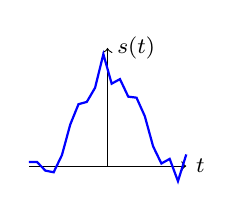
\begin{tikzpicture}
\draw[->] (0,0)--(0,1.5) node[right]{\footnotesize $s(t)$};
\draw[->] (-1,0)--(1,0) node[right]{\footnotesize $t$};
\draw[thick,blue] plot coordinates{(-5.00000/5,0.051378 )
 (-4.473684/5,0.051094) 
 (-3.947368/5,-0.057463)
 (-3.421053/5,-0.079000) 
 (-2.894737/5,0.139569)
  (-2.368421/5,0.526946)
   (-1.842105/5,0.786162) 
   (-1.315789/5,0.814761)
    (-0.789474/5,0.995006)
     (-0.263158/5,1.421068)
      (0.263158/5,1.046368)
       (0.789474/5,1.104432) 
       (1.315789/5,0.881924)
       (1.842105/5,0.868557) 
       (2.368421/5,0.633392)
        (2.894737/5,0.250564) (3.421053/5,0.032500) 
        (3.947368/5,0.091466) (4.473684/5,-0.191670) 
        (5.000000/5,0.147825) };
\end{tikzpicture}\\
\vspace{1cm}
\only<2->{
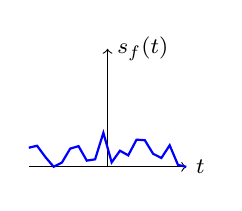
\begin{tikzpicture}
\draw[->] (0,0)--(0,1.5) node[right]{\footnotesize $s_f(t)$};
\draw[->] (-1,0)--(1,0) node[right]{\footnotesize $t$};
\draw[thick,blue] plot coordinates{
  (-1.0000e+00,  2.4316e-01)
  (-8.9474e-01,  2.6829e-01)
  (-7.8947e-01,  1.2528e-01)
  (-6.8421e-01,   1.6295e-03)
  (-5.7895e-01,   5.5155e-02)
  (-4.7368e-01,   2.3206e-01)
  (-3.6842e-01,  2.6316e-01)
  (-2.6316e-01,   7.9338e-02)
  (-1.5789e-01,   9.5695e-02)
  (-5.2632e-02,   4.3257e-01)
   (5.2632e-02,   5.7870e-02)
   (1.5789e-01,   2.0512e-01)
   (2.6316e-01,   1.4650e-01)
   (3.6842e-01,   3.4556e-01)
   ((4.7368e-01,   3.3851e-01)
   (5.7895e-01,   1.6615e-01)
   (6.8421e-01,   1.1313e-01)
   (7.8947e-01,   2.7421e-01)
   (8.9474e-01,   2.5521e-02)
   (1.0000e+00,   3.3961e-015)
 };
\end{tikzpicture}
}
\end{center}


\column{60mm}

 \begin{itemize}
 \item Supprimer des variations lentes non voulues
 \vspace{0.4cm}
 \item Faire ressortir les bords d'une image 
 
 \end{itemize}
\end{columns}
\end{frame}

\begin{frame}
\frametitle{Exemple d'utilisation : Filtre passe-haut}
\begin{columns}
\column{60mm}
\begin{center}
\includegraphics[width=50mm]{cells.png}
\end{center}

\column{60mm}
\only<2->{
\begin{center}
\includegraphics[width=50mm]{cells_sharp.png}
\end{center}
}
\end{columns}
\vspace{1cm}
\only<3->{
Le filtre passe-haut appliqué à l'image fait ressortir les bords \only<4->{$\rightarrow$ Segmentation }
}

\end{frame}

\begin{frame}
\frametitle{Types de filtres numériques : Phase} 
En terme de phase:
\begin{columns}
\column{60mm} 
\begin{itemize}
\item<2-> Phase linéaire \only<3->{ $\rightarrow$ Permet d'éviter les distorsions}
\vspace{0.6cm}

\item<4-> Phase quelconque 

\vspace{0.6cm}
\item<5-> Phase nulle \only<6-> { $\rightarrow$ Non causal}
\end{itemize}

\column{60mm}
\only<2->{
\begin{center}
\includegraphics[width=40mm]{lin_phase.png}
\end{center}
}

\end{columns}
\end{frame}

%\subsection{Ordre d'un filtre}
%\begin{frame}
%\frametitle{Ordre d'un filtre}
%Dans le cadre des filtres numériques
%
%\end{frame}


\subsection{Design de filtres: Contraintes}
\begin{frame}
\frametitle{Design de filtre}
Comment exprimer les contraintes relatives au design d'un filtre ?\\
\vspace{1cm}
Mots clés:
\begin{itemize}
\item<2->  Bande passante 
\vspace{0.3cm}
\item<3-> Fréquence de coupure
\vspace{0.3cm} 
\item<4->  Selectivité
\vspace{0.3cm}
\item<5-> etc...
\end{itemize}
\vspace{1cm}
\only<6->{
Toutes ces contraintes sont condensés dans un gabarit
}

\end{frame}

\begin{frame}
\frametitle{Design de filtre: Gabarit}
Exemple d'un gabarit d'un filtre passe bas filtre passe-bas:\\
\vspace{0.5cm} 
\begin{columns}
\column{60mm}
\begin{center}
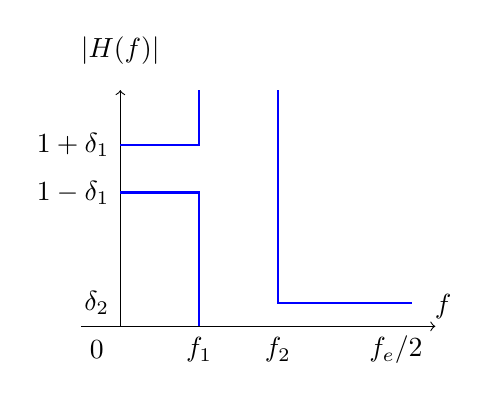
\begin{tikzpicture}

	\draw[->] (-0.5,0)-- (4,0);
\draw (-0.3,-0.3) node {0};
\draw[->] (0,0)-- (0,3);
\draw (4.1,0.25) node {$f$};
\draw (0,3.5) node {$|H(f)|$};
\draw (1,-0.3) node {$f_1$};
\draw (2,-0.3) node {$f_2$};
\draw (-0.6,1.7) node {$1 - \delta_1$};
\draw (-0.6,2.3) node {$1 + \delta_1$};
\draw (-0.3,0.3) node {$\delta_2$};
\draw (3.5,-0.3) node {$f_e/2$};


\draw[thick,blue](0,1.7)--(1,1.7)--(1,0);
\draw[thick,blue](0,2.3)--(1,2.3)--(1,3);
\draw[thick,blue](2,3)--(2,0.3)--(3.7,0.3);

\end{tikzpicture}
\end{center}

\column{60mm}
\begin{itemize}
\item<2-> $\delta_1$ : Tolérance en bande passante 
\vspace{0.2cm}
\item<3->$\delta_2$ : Tolérance en bande affiablie  
\vspace{0.2cm}
\item<4-> $f_1$ : fréquence de transition-bande passante 
\vspace{0.2cm}
\item<5-> $f_2$ : fréquence de transition-bande affaiblie 
\end{itemize}

\end{columns}
\end{frame}

\subsection{Réponse en fréquence : Deuxième exemple}

\begin{frame}
\frametitle{Réponse en fréquence: Deuxième exemple}
Réponse en fréquence du filtre: $H_2(z)  = \frac{\displaystyle  z}{ \displaystyle z-1 }$\\
\vspace{0.2cm}
\only<2->{
\underline{Remarque} : Ici le filtre comporte des termes en $z$ au dénominateur...\\
}
\vspace{0.3cm}
\only<3->{
\[H_2(z)  = \frac{z}{z-1 } \rightarrow H_2(\nu) = \frac{1}{2 e^{-\pi \nu T_e}   \sin (\pi \nu T_e)} =  \] 
}
\begin{columns}
\column{60mm}
\only<4->{
\[ |H_2(\nu)| = \frac{1}{2 |\sin(\pi \nu T_e)|} \] 
}
\column{60mm}
\only<4->{
\[ \textrm{arg}(H_2(\nu)) = -\arctan(\frac{1}{\tan( \pi \nu T_e)}) \]
} 
\end{columns}
\end{frame}

\begin{frame} 
\frametitle{Réponse en fréquence: Deuxième exemple}
Réponse en fréquence du filtre: $H_2(z)  = \frac{\displaystyle  z}{ \displaystyle z-1 }$\\
\vspace{0.2cm}

\begin{columns}
\column{60mm}
\only<2->{
\[ |H_2(\nu)| = \frac{1}{2 |\sin(\pi \nu T_e)|} \] 
}
\vspace{0.25cm}
\only<3->{
\begin{center}
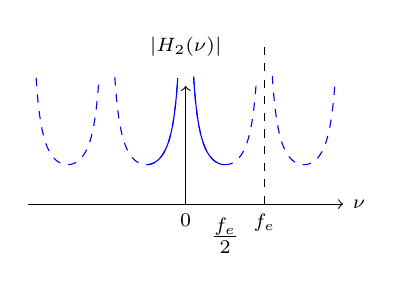
\begin{tikzpicture}
\draw[->] (-2,0)--(2,0) node[right] { $\scriptstyle \nu$};
\draw[->] (0,0)node[below] {\scriptsize 0} -- (0,1.5) ;
\draw (0,2) node {$\scriptstyle |H_2(\nu)|$};
\draw (0.5,-0.4) node {$\frac{f_e}{2}$};

\draw[domain=0.1:0.5,color=blue,samples=100] plot (\x,{1/(2*abs(sin(3.14 *\x r)))});
\draw[dashed,domain=0.1:0.9,color=blue,samples=100] plot (\x,{1/(2*abs(sin(3.14 *\x r)))});
\draw[dashed,domain=1.1:1.9,color=blue,samples=100] plot (\x,{1/(2*abs(sin(3.14 *\x r)))});

\draw[domain=-0.5:-0.1,color=blue,samples=100] plot (\x,{1/(2*abs(sin(3.14 *\x r)))});
\draw[dashed,domain=-0.9:-0.1,color=blue,samples=100] plot (\x,{1/(2*abs(sin(3.14 *\x r)))});
\draw[dashed,domain=-1.9:-1.1,color=blue,samples=100] plot (\x,{1/(2*abs(sin(3.14 *\x r)))});

\draw[dashed](1,0) node[below]{\scriptsize $f_e$}--(1,2);
\end{tikzpicture}
\end{center}
}
\column{60mm}
\only<2->{
\[ \textrm{arg}(H_2(\nu)) = -\arctan(\frac{1}{\tan( \pi \nu T_e)}) \]\\
} 
\vspace{0.4cm}
\only<3->{
\begin{center}
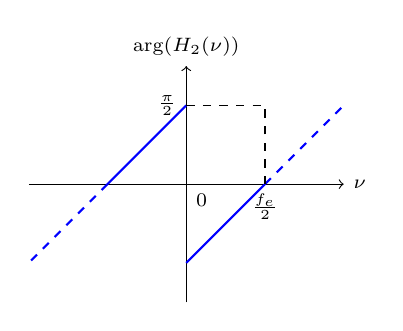
\begin{tikzpicture}
\draw[->] (-2,0)-- (2,0) node[right] {$\scriptstyle \nu$};
\draw[->] node[below right]{\scriptsize 0} (0,-1.5) -- (0,1.5) node[above] {$\scriptstyle \textrm{arg}(H_2(\nu))$} ;


\draw[thick,blue] (0,-1)--(1,0);
\draw[thick,blue] (-1,0)--(0,1); 
\draw[dashed,thick,blue] (1,0)--(2,1); 
\draw[dashed,thick,blue] (-1,0)--(-2,-1); 

\draw[dashed] (1,0) node[below] {$\scriptstyle \frac{f_e}{2}$} --(1,1) ;
\draw[dashed] (0,1) node[left] {$\scriptstyle \frac{\pi}{2}$} --(1,1)  ; 
\end{tikzpicture}
\end{center}
}
\end{columns}
\vspace{0.2cm}
\only<4->{
Le filtres est \textbf{instable} aux fréquences multiples de $f_e$... 
}

\end{frame}

\subsection{Notion de récursivité, pôles et zéros}
\begin{frame}
\frametitle{Notion de récursivité}
Au-delà des caractéristiques fréquentielles deux grandes classes de filtres numériques existent : \\
\vspace{0.2cm}
\begin{columns}[T]
\column{60mm}
Filtre non-récursifs:\\
\vspace{0.3cm}
\only<2->{
\begin{center}
	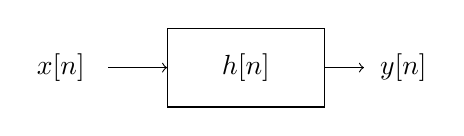
\begin{tikzpicture}
	\draw (2.15,0) node {$x[n]$};
	
	\draw[->] (2.75,0)-- (3.5,0);
	\draw (3.5,-0.5) rectangle(5.5,0.5) ;
	\draw (4.5,0) node {$h[n]$};
	
	\draw[->] (5.5,0)-- (6,0);

	\draw (6.5,0) node {$y[n]$};
	%\draw (4.5,-2) node {filtre non-récursif};
\end{tikzpicture}
\end{center}
}
\vspace{0.8cm}	
\only<3->{
\[ H(z) = 1+ a_1 z + a_2 z^2 + \cdots + a_n z^n  \] 
}	 

\column{60mm}
Filtre récursifs: \\
\vspace{0.3cm}
\only<2->{
\begin{center}
	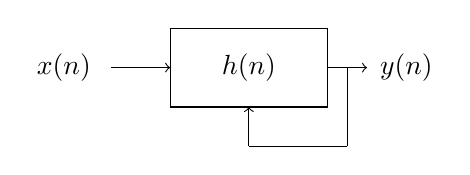
\begin{tikzpicture}
	\draw (2.15,0) node {$x(n)$};

	
	\draw[->] (2.75,0)-- (3.5,0);
	\draw (3.5,-0.5) rectangle(5.5,0.5) ;
	\draw (4.5,0) node {$h(n)$};
	
	\draw[->] (5.5,0)-- (6,0); 
	\draw (6.5,0) node {$y(n)$};

	%\draw (4.5,-2) node {filtre récursif};
	
	\draw[-] (5.75,0)-- (5.75,-1);
	\draw[-] (5.75,-1)-- (4.5,-1);
	\draw[->] (4.5,-1)-- (4.5,-0.5);
	\end{tikzpicture}
\end{center}
}
\vspace{0.2cm}
\only<3->{
\[ H(z) = \frac{1+ a_1 z + a_2 z^2 + \cdots + a_n z^n }{1+ b_1 z + b_2 z^2 + \cdots + b_n z^n} \] 
}

\end{columns} 

\end{frame}

\subsection{Pôles et zéros}
\begin{frame}
\frametitle{Notion de pôles et de zéros}
Soit une fonction de transfert d'un système récursif: \\
\[ H(z) = \frac{1+ a_1 z + a_2 z^2 + \cdots + a_n z^n }{1+ b_1 z + b_2 z^2 + \cdots + b_n z^n} = \frac{(z-z_1)(z-z_2)...(z-z_n)}{(z-p_1)(z-p_2)...(z-p_n)} \] 

\vspace{0.3cm}

\begin{columns}[T]
\column{60mm}
zéros : ensemble des $z_n$ \\
\begin{itemize}
\item<3-> annule la fonction de transfert
\item<4-> filtres récursifs et non-récursifs 
\end{itemize}
\column{60mm}
pôles : ensemble des $p_n$ \\
\begin{itemize}
\item<3-> fait diverger la fonction de transfert
\item<4-> filtre récursifs uniquement
\end{itemize}

\end{columns} 

\end{frame}

\begin{frame}
\frametitle{Plan pôle-zéro}
La notion de plan pôle zéro existe aussi pour la transformée en z\\
\vspace{0.2cm}
\begin{columns}
\column{60mm}
Laplace:
\begin{center}
	\begin{tikzpicture}
	\draw[->] (-2,0)--(2,0) node[right]{Re($s$)};
	\draw[->] (0,-2)--(0,2)node[above]{Im($s$)};
	
	\only<2->
	{
		\draw[->,thick,blue] (0,-2)--(0,2);
		\draw[fill=blue,opacity=0.2] (-2,-2) rectangle(0,2) ;
		\draw[<-,blue] (-0.5,-1)--(2.5,-1) node[blue,right] {zone de stabilité};
	}
	
		\only<3->
	{
		\draw (1,0) node{o};
		\draw (1,-0.4) node{\footnotesize zéro};
		\draw (-1.2,-1) node{x};
		\draw (-1.2,1) node{x};
		\draw[dashed] (-1.2,-1)--(-1.2,1) ;
	}
	\end{tikzpicture}
\end{center}
	
\column{60mm}
z:
\begin{center}
	\begin{tikzpicture}
		\draw[->] (-2,0)--(2,0) node[right]{Re($z$)};
	\draw[->] (0,-2)--(0,2)node[above]{Im($z$)};
		
	
	\only<2->
	{
		\draw[blue,fill=blue,opacity=0.2] (0,0) circle (1);
		\draw[blue,thick] (0,0) circle (1);
		\draw[->,blue] (-2,-1)--(-0.5,-0.3);
	}
	
	\only<3->
	{
		\draw (1,0) node{o};
		\draw (-0.5,0.6) node{x};
		\draw (-1,0.9) node{\footnotesize pôle stable};
		\draw (-0.5,-0.6) node{x};
		\draw[dashed] (0,0)--(-0.5,-0.6);	
		\draw[dashed] (0,0)--(-0.5,0.6);		
	}
	\end{tikzpicture}
\end{center}

\end{columns} 
\vspace{0.3cm}
Coeffs réels $\rightarrow$ pôles doubles et réels ou complexes conjugués
\end{frame}

\begin{frame}
\frametitle{Résumé du chapitre}
\begin{enumerate}
\item Définitions
\begin{itemize}
\item Fonction de transfert 
\vspace{0.1cm}
\item \'Equation de récurrence
\vspace{0.1cm}
\item Réponse impulsionnelle
\vspace{0.1cm}
\end{itemize}
\vspace{0.2cm} 
\item Types de filtres \& Gabarit  :
\begin{itemize}
\item Passe-bas
\vspace{0.1cm}
\item Passe-haut
\vspace{0.1cm}
\item Passe-bande
\vspace{0.1cm}
\item Coupe-bande
\end{itemize}
\vspace{0.2cm} 
\item Récursivité, pôles et zéros :
\begin{itemize}
\item Définitions pôle et zéros
\vspace{0.1cm}
\item Graphe pôle-zéro
\end{itemize}
\vspace{0.2cm} 

\end{enumerate}
\end{frame}


\begin{frame} 
\frametitle{Structure du cours}
\vspace{0.3cm}
\begin{enumerate}
\item Outils mathématiques généraux  
\vspace{0.3cm}
\item Signaux numériques  
\vspace{0.3cm}
\item Filtres numériques : Généralités 
\vspace{0.3cm}
\item Filtres récursifs et méthodes de synthèse
\vspace{0.3cm}
\item Filtres non-récursifs et méthodes de synthèse
\vspace{0.3cm}
\item Signaux Biomédicaux
\vspace{0.3cm}
\item Application : Détection complexe QRS
\vspace{0.3cm}
\item Ultrasons Doppler
\vspace{0.3cm}
\item Application Doppler: Détection embolie gazeuse veineuse
\end{enumerate}
\end{frame} 



\end{document}
